%%
%% aim_and_objectives.tex
\forcecommand{\thesec}{Aim and Objectives}
\section{\thesec}
\label{sec:aim_and_objectives}
%%

%%
%% aim:
%%   what is the main expected outcome of your research? 
%%   what would you like to accomplish (in concrete terms)?
\begin{frame}{\thesec}{}
  \vspace{-2\baselineskip}
  \begin{block}{Aim}
    \begin{itemize}
      \item{
        To develop (more precisely: adapt) CFD code capable of simulating the breakup of liquid jets and sheets, particularly in cases involving impact with a solid surface.
      }
    \end{itemize}
  \end{block}
  \begin{figure}
    \centering
    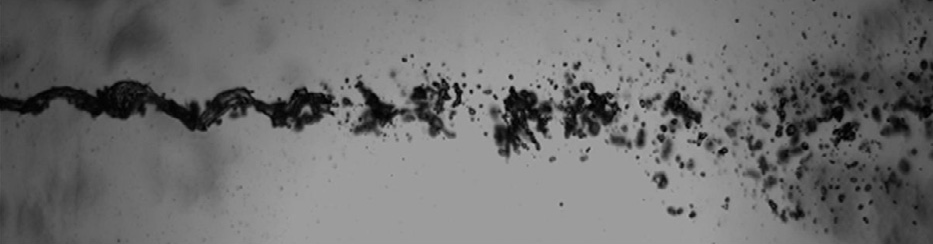
\includegraphics[width=\textwidth]{img/flappingSheetBreakup12300.png}
    \caption{From Ren, Marshall, 2014 {\color{white}\cite{Ren14}}}
  \end{figure}
\end{frame}

%%
%% objectives:
%%   what specific steps will you take to achieve your aim?
\begin{frame}{\thesec}{}
  \vspace*{-2\baselineskip}
  \begin{block}{Objectives}
    \begin{itemize}
      \item{ choose appropriate CFD method }
      \item{ develop simulation software based on CFD method }
      \item{ validate against data from physical experiments }
    \end{itemize}
  \end{block}
  \begin{block}{Data of interest:}
    \begin{itemize}
      \item{ velocity distribution of spray droplets }
      \item{ distribution of liquid water content (LWC) in spray cloud }
      \item{ size distribution of spray droplets }
    \end{itemize}
  \end{block}
\end{frame}

%%
%% why model spray generation? what's wrong with the way things are currently done?
\forcecommand{\thesec}{Motivation}
%%
\begin{frame}{\thesec}{}
  \vspace*{-2\baselineskip}
  \begin{block}{Benefits of simulating the spray generation process:}
    \begin{itemize}
      \item{
        no calibration of empirical parameters required
      }
      \item{
        applicability under general circumstances (superstructure geometries, weather conditions, etc.)
      }
	  \item{
	    ability to predict spray cloud behavior on existing vessels and superstructures based on weather conditions, allowing for the development of vessel- or superstructure-specific icing forecasts
	  }
	  \item{
	    ability to predict spray cloud behavior for vessels and superstructures of arbitrary geometry while still in the design phase, allowing for the inclusion of anti-icing measures in potential problem areas
	  }
    \end{itemize}
  \end{block}
\end{frame}
%% M. Sullivan. June, 2016